\begin{frame}{Symulowane wyżarzanie [ang. \textit{Simulated Annealing}]}

	\begin{block}{}
	Rodzaj algorytmu heurystycznego przeszukującego przestrzeń alternatywnych rozwiązań problemu w celu wyszukiwania rozwiązań najlepszych. Jest wariantem metody przeszukiwania lokalnego [ang. \textit{Local Search}].
	Ogólny szkic działania algorytmu symulowanego wyżarzania:
	\end{block}
	\begin{enumerate}
		\item losowy wybór punktu startowego
		\item losowy wybór sąsiada
		\item odpowiednia akceptacja sąsiada
		\item po każdej iteracji temperatura zostaje zaktualizowana:
			$$ T = n\cdot T \wedge n \in (0,1)$$
		\item algorytm zatrzymuje się gdy w ciągu ustalonej liczby iteracji nie uda się osiągnąć lepszego wyniku
	\end{enumerate}

\end{frame}

\begin{frame}{Symulowane wyżarzanie [ang. \textit{Simulated Annealing}]}

    \begin{algorithmic}[H]
    \State $n -- \ \text{dlugosc permutacji}$
    \While{$k = 0 to n^3$}{
    }
    \end{algorithmic}
	\scalebox{0.4}{
	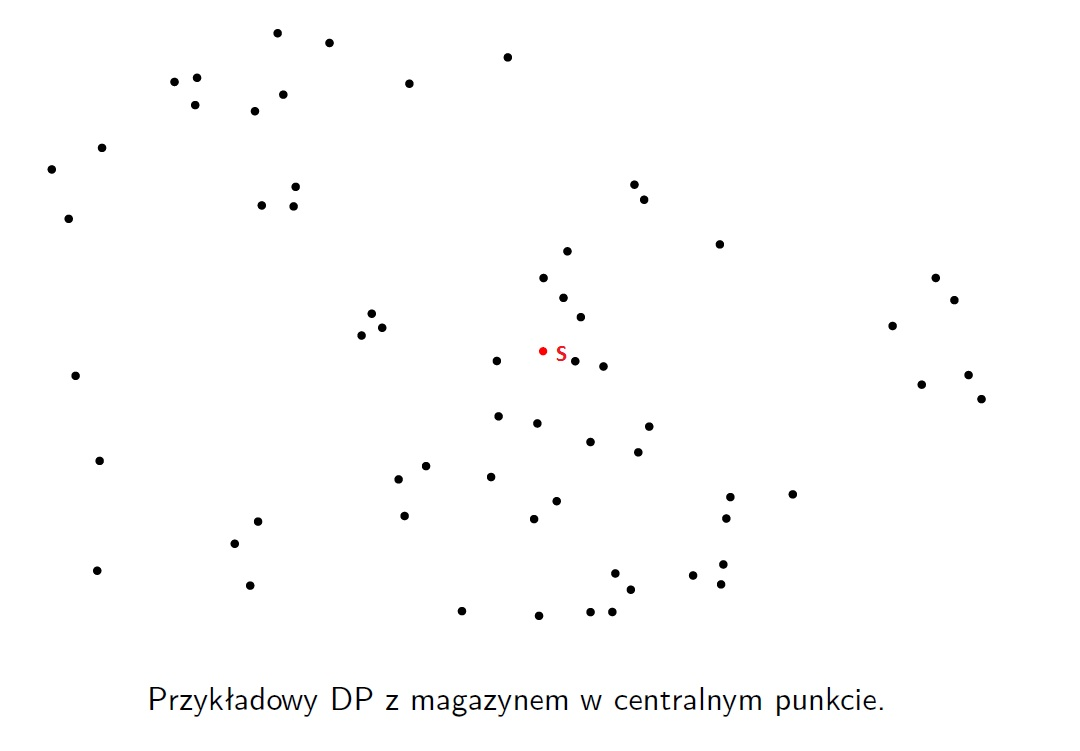
\includegraphics{./slajdy/1.jpg}}

\end{frame}

\begin{frame}{Symulowane wyżarzanie [ang. \textit{Simulated Annealing}]}

	\scalebox{0.4}{
	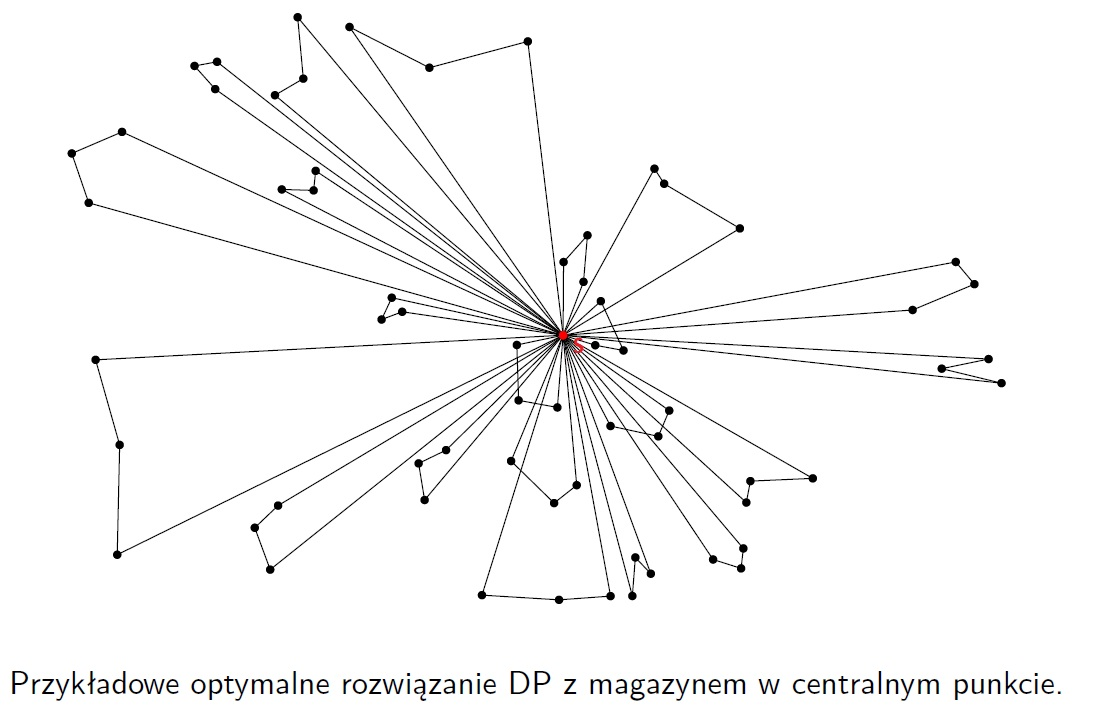
\includegraphics{./slajdy/2.jpg}}

\end{frame}

\begin{frame}{Symulowane wyżarzanie [ang. \textit{Simulated Annealing}]}
	
	\scalebox{0.4}{
	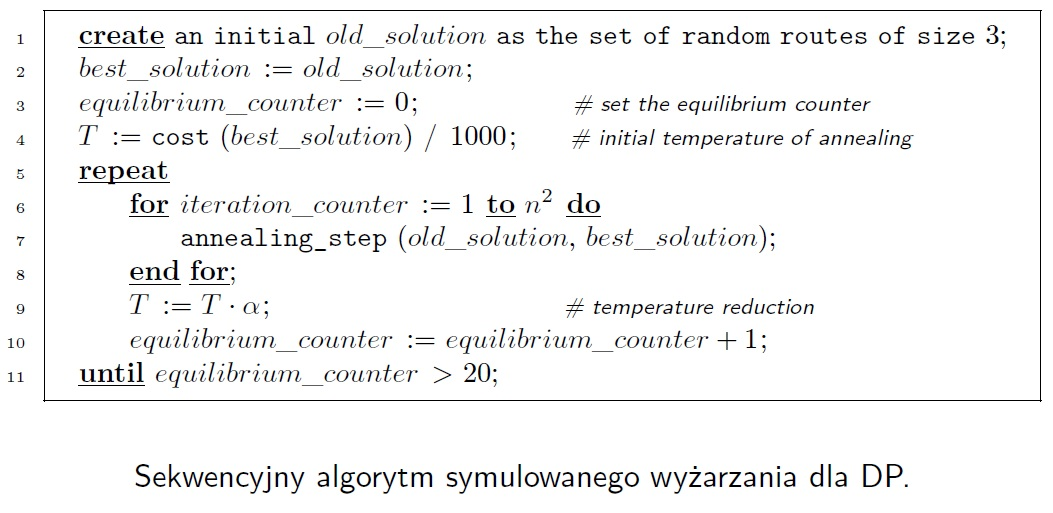
\includegraphics{./slajdy/3.jpg}}

\end{frame}

\begin{frame}{Symulowane wyżarzanie [ang. \textit{Simulated Annealing}]}

	\scalebox{0.4}{
	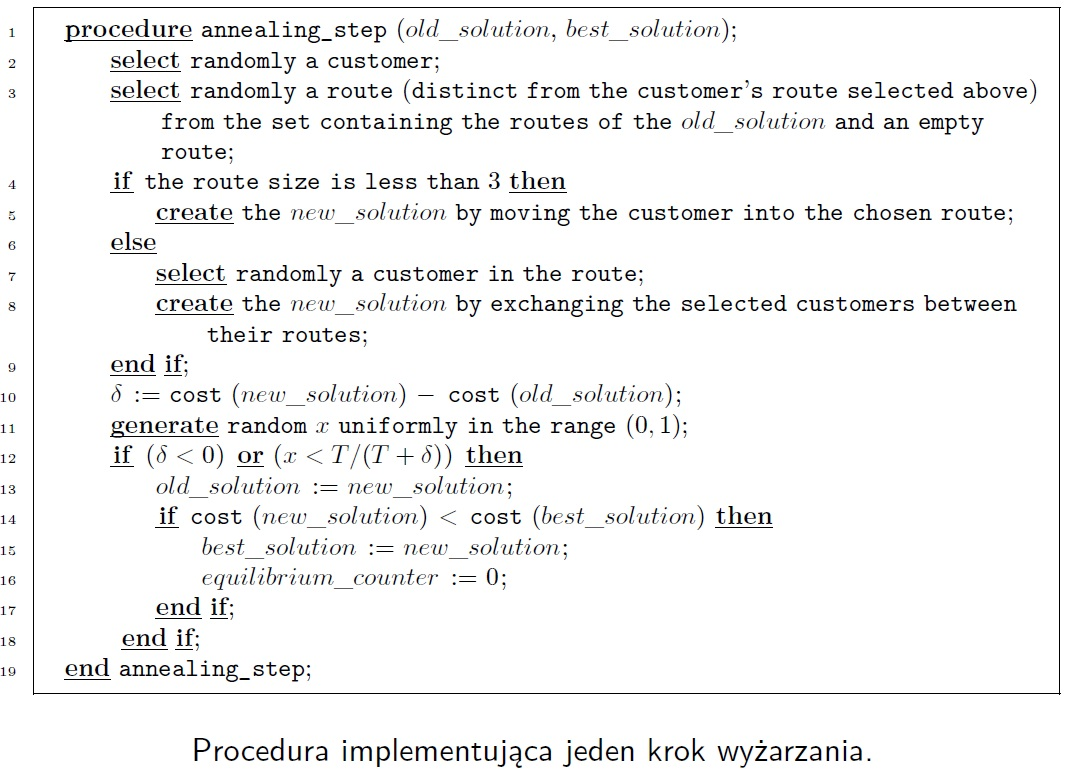
\includegraphics{./slajdy/4.jpg}}

\end{frame}
